\documentclass[12pt]{article}
\usepackage{graphicx} % Required for inserting images

\title{Computer Project 1: Comparing Analytic and Finite-Difference Numerical solutions to a transient system}
\author{Owen Strong \\
\itshape Prof.: Caleb Brooks
}
\date{March 4th, 2026}

\usepackage[
    style=ieee
]{biblatex}
\bibliography{refs.bib}

\usepackage[letterpaper, margin=1in]{geometry}
\newcommand{\figwidth}{0.75\linewidth}

% Common Macros
\newcommand{\micCi}{~$\mathrm{\mu Ci}$~}

\usepackage{placeins} % FloatBarrier
\usepackage{amsmath} % align
\usepackage{xcolor}
\usepackage[colorlinks=true, citecolor=violet, linkcolor=violet, urlcolor=violet]{hyperref}
\usepackage{enumitem}

\begin{document}
\pagenumbering{gobble}
\maketitle
\pagebreak
{\hypersetup{linkcolor=black}\tableofcontents}
\pagenumbering{arabic}
\begin{abstract}

\end{abstract}

\section{Introduction and Background}
\FloatBarrier
Heat transfer is a critical phenomenon to understand in virtually any engineering field, from the cooling of spacecraft in vacuum to the power generation of a nuclear reactor to simply saving money heating a house during winter.\\

Temperature is a macroscopic phenomenon, describing the average kinetic energy of particles within a medium (as opposed to the bulk motion of the medium).
Heat transfer, then, is the thermal energy in transit caused by a spacial difference in temperature.
Heat transfer may be understood as a combination of three empirical phenomena: conduction, convection, and radiation, shown in Fig.~\ref{fig:intr-modes}.
Of these, conduction and convection will be the primary interest in this report.\\

\begin{figure}
    \centering
    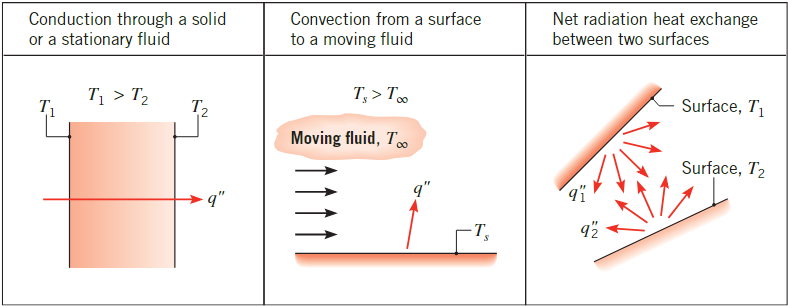
\includegraphics[width=\figwidth]{fig/intr0_modes.png}
    \caption{Conduction, convection, and radiation heat transfer modes. Figure sourced from \textit{Fundamentals of Heat and Mass Transfer}.\cite{bergman_fundamentals_2017}}
    \label{fig:intr-modes}
\end{figure}

Conduction, in which thermal energy diffuses through particles in the medium, follows Fourier's law:
\begin{equation}
    \vec{q''}_{cond}=-k\nabla T
\end{equation}
where $\vec{q''}_{cond}$ is the directional heat flux (i.e. heat transfer per unit area) caused by conduction, $\nabla T$ is the temperature gradient, and $k$ is \emph{thermal conductivity}, a material property relating the two.\\

Convection, in which conduction is combined with bulk motion of a fluid, is described for a surface interface between a material and the fluid, using Newton's law of cooling:
\begin{equation}
    \vec{q''}_{conv}=h(T_f - T_s)
\end{equation}
Where $T_f$ is the temperature of the convective fluid, $T_s$ the temperature at the surface, and $\vec{q''}_{cond}$ is the directional heat flux resulting from this convection.\\

Fourier's law of conduction can be related to a control volume to derive the General Heat Diffusion Equation (GHDE) for a particular location within a material\cite{bergman_fundamentals_2017}:
\begin{equation}
    \rho c_p\frac{\partial T}{\partial t} = -\nabla k \nabla T + q''' 
\end{equation}
where $\rho$ represents mass density and $c_p$ the heat capacity of the material, and $q'''$ the volumetric heat generation at that location.
For a material with uniform properties, this is typically simplified to:
\begin{equation}\label{eq:ghde-alpha}
    \frac{1}{\alpha}\frac{\partial T}{\partial t} = \frac{q'''}{k} - \nabla^2T
\end{equation}
where $\alpha$ is the thermal diffusivity of the material: \\
\begin{equation}
    \alpha = \frac{k}{\rho c_p}
\end{equation}

This equation, in either form, can be solved analytically.
However, doing so in cases considering anything more than one dimension (including considering time) is non-trivial, and quickly devolves into tedious calculus including summations of eigenfunctions.\cite{bergman_fundamentals_2017}\\

For a transient one-dimensional problem (one with time dependence), there are two immediate techniques to avoid this analysis: the lumped sum approximation, and a numerical simulation.

In this report, an analytic solution using the lumped sum approximation will be compared to a finite difference numerical solution, for a problem involving a uniform sphere subjected to convection in a cooling fluid.
\FloatBarrier\subsection{Lump Sum Approximation}
Consider a uniform sphere which is highly conductive, subjected to convective cooling by a fluid surrounding it.
One could solve for the temperature distribution within the sphere over time using Equation~\ref{eq:ghde-alpha}, but if the sphere is highly conductive (high $k$) compared to the convective ability of the fluid and surface (low $h$), then one can instead assume a uniform temperature $\bar{T}$ over the surface.
Applying a control volume around the sphere, uniform over its volume $V$, with a surface area $A$ in contact with the fluid:
\begin{equation}\label{eq:lumped}
    \rho c_pV\frac{d\bar{T}(t)}{dt} = -hA(\bar{T}(t) - T_f) + q'''
\end{equation}
This equation, which now only considers one variable, can be solved by changing perspective to the relative temperature $\bar{\theta}=\bar{T} - T_f$ (assuming heat generation $q'''=0$):
\begin{gather*}
    \rho c_pV\frac{d\bar{\theta}}{dt} = -hA(\bar{\theta}) + q'''\\
    \frac{d\bar{\theta}}{dt}=-\frac{hA}{\rho c_p V}\bar{\theta}\\
    \frac{1}{\bar{\theta}}d\bar{\theta} = -\frac{hA}{\rho c_p V}dt\\
    \ln(\bar{\theta}) = -\frac{hA}{\rho c_p V}t + C\\
    \color{gray}\rightarrow \tau=\frac{hA}{\rho c_p V}\\
    \ln(\bar{\theta}) = -\frac{t}{\tau} + C\\
    \bar{\theta}=Ce^{-\frac{t}{\tau}}\\
    \color{gray}\rightarrow \bar{\theta}(t=0)=\bar{\theta_0}\\
    \bar{\theta_0}=Ce^{-\frac{0}{\tau}}=C\\
    \boxed{\bar{\theta}=\bar{\theta_0}e^{-\frac{t}{\tau}}}
\end{gather*}

If one component out of the material properties contained in the time constant $\tau$, the initial temperature difference $\bar{\theta_0}$, the time $t$, or the temperature difference $\bar{\theta}$ at that time, this equation can be used to solve for the missing value of otherwise known system, such as the convection coefficient necessary in a fluid for a given conductive sphere to go from an initial temperature to a known final temperature within that fluid after a known time.\\

To consider whether it is appropriate to use the lumped sum approximation, the Biot number, a dimensionless quantity relating thermal convection to conduction, should be appropriately low:
\begin{equation}
    \label{eq:biot}
    B_i=\frac{hL}{k}\leq0.1
\end{equation}
where $L$ is the characteristic length of the system in question, in this case the diameter of the sphere, and $k$ and $h$ the conductive material's conductivity and the fluid-material interface's convection coefficient, respectively.

\FloatBarrier\subsection{Finite Difference}
If, instead, one discretizes Equation~\ref{eq:ghde-alpha} (once again assuming no heat generation) over finite differences in time ($t=p\Delta t$) and the radius of the sphere ($r=n\Delta r$):
\newcommand{\btheta}{\bar{\theta}}
\begin{gather*}
    \frac{1}{\alpha}\frac{\partial T}{\partial t} = \frac{q'''}{k} - \nabla^2T\\
    \frac{1}{\alpha}\frac{\partial \btheta}{\partial t} = - \frac{1}{r^2}\frac{d}{dr}\left(r^2\frac{d\btheta}{dr}\right)\\
    \frac{1}{\alpha}\frac{\partial \btheta}{\partial t} = - \frac{1}{r^2}\frac{d}{dr}\left(n^2\Delta r^2\frac{T_{n+\frac{1}{2}} - T_{n-\frac{1}{2}}}{\Delta r}\right)\\
    \frac{1}{\alpha}\frac{\partial \btheta}{\partial t} = - \frac{1}{r^2}\frac{d}{dr}\left(n^2\Delta r({T_{n+\frac{1}{2}} - T_{n-\frac{1}{2}}})\right)\\
    \frac{\partial \btheta}{\partial t} = \frac{\alpha}{\Delta r^2} \frac{(n+\frac{1}{2})^2[T_{n+1}-T_n] - (n-\frac{1}{2})^2[T_n-T_{n-1}]}{n^2}
\end{gather*}
discretizing over time such that the gradient is evaluated at the previous timestep $p$ (\emph{``explicit''} finite difference) and introducing the differential system's Fourier number $F_o$:
\begin{gather*}
    \frac{\partial \btheta}{\partial t} = \frac{\alpha}{\Delta r^2} \frac{(n+\frac{1}{2})^2[T_{n+1}-T_n] - (n-\frac{1}{2})^2[T_n-T_{n-1}]}{n^2}\\
    \frac{T_n^{p+1} - T_n^p}{\Delta t} = \frac{\alpha}{\Delta r^2} \frac{(n+\frac{1}{2})^2[T_{n+1}^p-T_n^p] - (n-\frac{1}{2})^2[T_n^p-T_{n-1}^p]}{n^2}\\
    \frac{T_n^{p+1} - T_n^p} = \frac{\alpha\Delta t}{\Delta r^2} \frac{(n+\frac{1}{2})^2[T_{n+1}^p-T_n^p] - (n-\frac{1}{2})^2[T_n^p-T_{n-1}^p]}{n^2}\\
    \color{gray}\rightarrow F_o = \frac{\alpha \Delta t}{\Delta r^2}\\
    {T_n^{p+1} - T_n^p} = F_o \frac{(n+\frac{1}{2})^2[T_{n+1}^p-T_n^p] - (n-\frac{1}{2})^2[T_n^p-T_{n-1}^p]}{n^2}
\end{gather*}
\begin{equation}
    \label{eq:efd}
    T_n^{p+1} = T_n^p + F_o \frac{(n+\frac{1}{2})^2[T_{n+1}^p-T_n^p] - (n-\frac{1}{2})^2[T_n^p-T_{n-1}^p]}{n^2}
\end{equation}
By selecting offset indices of $n\in\{\frac{1}{2}, \frac{3}{2}, \frac{5}{2}...\}$, one may dictate a symmetric boundary condition where no heat passes through the center of the sphere, making the node $n=\frac{1}{2}$ only dependent on its outer neighbor $\frac{3}{2}$:
\begin{gather*}
    T_n^{p+1} = T_n^p + F_o \frac{(n+\frac{1}{2})^2[T_{n+1}^p-T_n^p] - (n-\frac{1}{2})^2[T_n^p-T_{n-1}^p]}{n^2}\\
    \color{gray}\rightarrow n=\frac{1}{2}\\
    T_n^{p+1} = T_n^p + F_o \frac{(1)^2[T_{n+1}^p-T_n^p] - (0)^2[T_n^p-T_{n-1}^p]}{\frac{1}{2}^2}\\
    T_{\frac{1}{2}}^{p+1} = T_{\frac{1}{2}}^p + F_o \frac{T_{\frac{3}{2}}^p-T_{\frac{1}{2}}^p}{\frac{1}{2}^2}\\
\end{gather*}
And, for the outermost node $n_s$ placed exactly at the surface of the sphere meeting the convective fluid, applying a control volume meeting the previous node at the internal conducting control surface $n_s-\frac{1}{2}$:
\newcommand{\note}{\color{gray}\rightarrow}
\begin{gather*}
    \frac{V_{n-\frac{1}{2},n}\rho c_p}{\delta t}(T_n^{p+1} - T_n^p)=kA_{n-\frac{1}{2}}\frac{T_{n-1}^p-T_n^p}{\Delta r} + hA_n(T_f-T_n^p)\\
    \note V_{n-\frac{1}{2},n} = \frac{4}{3}\pi (n^3-(n-\frac{1}{2})^3)\\
    \note A_n = 4\pi n^2\\
    T_n^{p+1} - T_n^p = 3F_o\frac{(n-\frac{1}{2})^2}{n^3-(n-\frac{1}{2})^3}(T_{n-1}^p-T_n^p) + 3F_oB_i\frac{n^2}{n^3-(n-\frac{1}{2})^3}(T_f-T_n^p)\\
    % T_n^{p+1} = (1-3F_o\frac{(n-\frac{1}{2})^2}{n^3-(n-\frac{1}{2})^3}-3F_oB_i\frac{n^2}{n^3-(n-\frac{1}{2})^3})T_n^p + 3F_o\frac{(n-\frac{1}{2})^2}{n^3-(n-\frac{1}{2})^3}T_{n-1}^p + 3F_oB_i\frac{n^2}{n^3-(n-\frac{1}{2})^3}T_f
\end{gather*}
or more concisely, by establishing dimensionless internal and edge geometric attenuation coefficients $\Gamma_i=\frac{(n_s-\frac{1}{2})^2}{n_s^3-(n_s-\frac{1}{2})^3}$, $\Gamma_e=\frac{n_s^2}{n_s^3-(n_s-\frac{1}{2})^3}$
\begin{equation}
    \label{eq:fd-surface}
    T_{n_s}^{p+1} = (1-3F_o\Gamma_i-3F_oB_i\Gamma_e)T_{n_s}^p + 3F_o\Gamma_iT_{n_s-1}^p + 3F_oB_i\Gamma_eT_f
\end{equation}
As ensuring stability requires a positive coefficient of the current temperature $T_n^p$, this yields a strict stability criterion:
\begin{equation}
    \label{eq:stability}
    \frac{1}{3}\geq F_o(\Gamma_i + B_i\Gamma_e)
\end{equation}
Since in Equation~\ref{eq:stability}, the characteristic length and time in $F_o$ and $B_i$ correspond to the differential length $\Delta r$ and time $\Delta t$, $B_i$ (only dependent on geometry) can be used to solve for the required $F_o$,
\begin{equation}
   F_o \leq \frac{1}{3 (\Gamma_i + B_i\Gamma_e)} 
\end{equation}
then solved for the maximum stable timestep $\Delta t$:
\begin{gather*}
    \frac{\alpha \Delta t}{\Delta r^2}\leq \frac{1}{3 (\Gamma_i + B_i\Gamma_e)}\\
    \boxed{\Delta t \leq \frac{\Delta r^2}{3\alpha (\Gamma_i + B_i\Gamma_e)}}
\end{gather*}

\section{Experimental Procedure}\label{sec:methods}
\section{Experimental Results}\label{sec:results}
\section{Discussion}\label{sec:disc}
\section{Conclusions}\label{sec:conc}

% \bibliographystyle{sty/ieeetran}
\printbibliography
\end{document}
